

\subsection{Community detection}


\subsubsection{Modularity maximisation}

In this work the authors \cite{Sobolevsky2022-di} compare Louivan \cite{Blondel2008-ik} and Leiden to Graph Neural Networks.

% Leiden
\paragraph*{Leiden algorithm}

% Louivan

\paragraph*{Constant Pots Model}

% Info Map

% The Markov thing
% SBM

% hSBM


\subsubsection{A generative approach}

\paragraph*{Stochastic Block Model}

The paper \cite{Peixoto2023-rt} is the culmination of the previous work done by Tiago's group and especially the work on comparing the descriptive and inferential algorithms. The main takeaway is that the authors in this paper demonstrated that the modularity maximisation methods are a special case of generative models and that these can be compared. It also compute the description lengths for each type which is then used as a metric. This is an improvement as previously \citet{Peixoto2021-jx} comparison was made by community sizes. Another point of the paper is that the non-parametric SBM (nSBM) \cite{Peixoto2014-yb} yields goods results compared with the others.

\begin{figure}[!htb]    
    \centering
    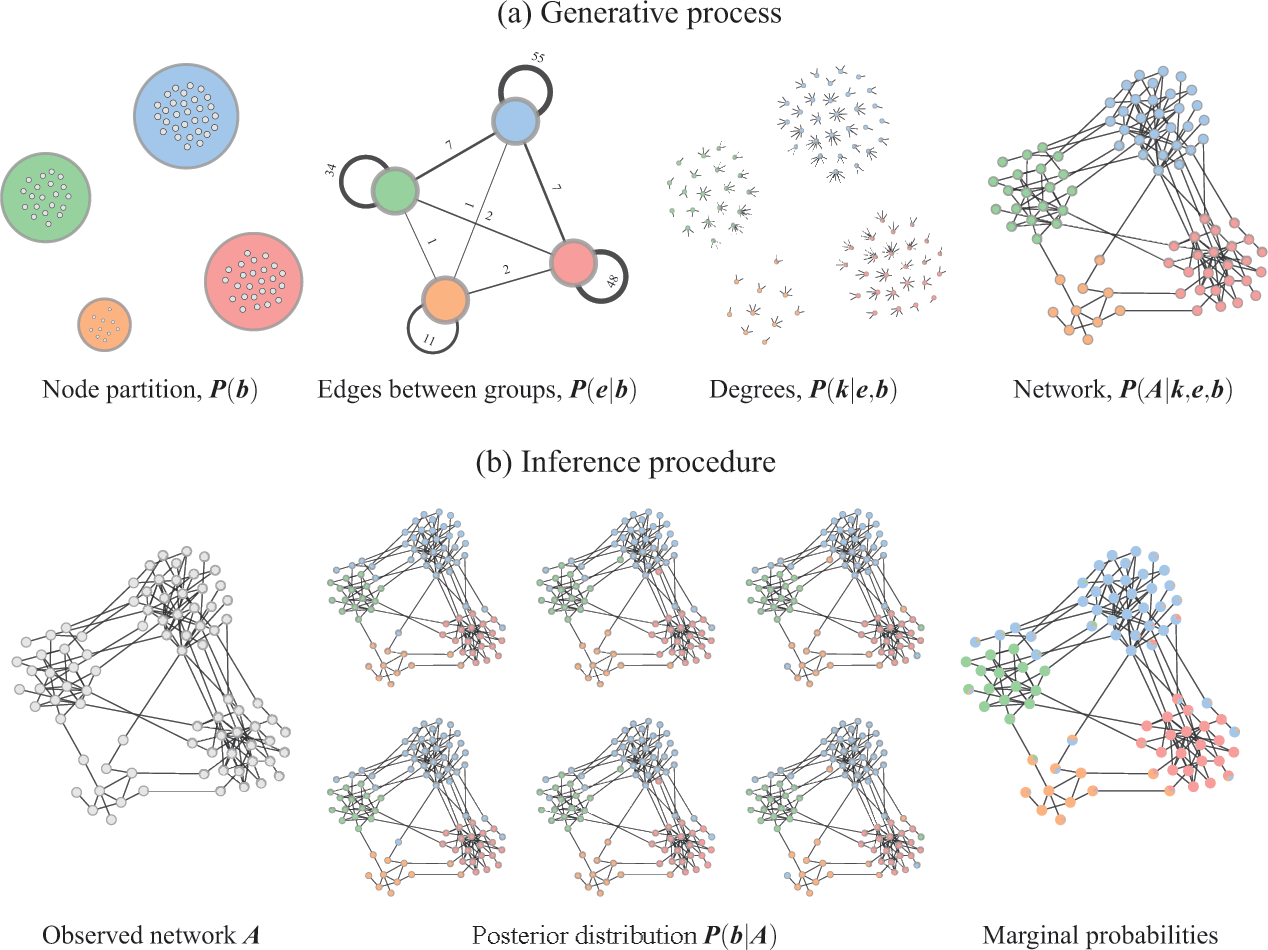
\includegraphics[width=1.0\textwidth,height=1.0\textheight,keepaspectratio]{Sections/Network_I/Resources/dc-sbm_explained.png}
    \caption{SBM explained. This is Figure 3 from \citet{Peixoto2021-jx}}
    \label{fig:N_I:dc-sbm_explained}
\end{figure}

There is a good description of the degree corrected SBM version in Figure \ref{fig:N_I:dc-sbm_explained}. For a node partition, $P(B)$ the network may be divided into 4 different communities. Each of these communities will have nodes that are connected inside (in-degree) or/and outside of the partition (out-degree); this is given by $P(e|b)$, where e is a matrix that specify how many edges go between groups r and s. Then, inside of each module, it can be looked at the individual nodes and their connections (degree), which is given by $ P(k|e,b)$; in the network before last it can be seen the un-connected nodes which are known as “stubs” or “half-edges”. With all this information, the nodes are connected and formed the observed network. Different partitions are generated and chosen the ones which held the best results according to the minimum description length.

\begin{equation} \label{eq:sbm}
         P(b|A) = \frac{P(A|b)P(b)}{P(A)}
\end{equation}

How well the partition b represent the network is measured by the description length, which is using concepts from Information Theory; i.e. how much information is needed to describe the network through likes of entropy. Lower information means is desired as the network is more ordered; i.e. that more ‘rules’ that generally describes the trends in the graph. More information needed, means that  when reconstructing the graph we need more information to do that. As it expected, for more communities there is a need for more information to describe the network. The author noted that this process is very similar to information compression.

\subsubsection{Summary}

\paragraph*{Descriptive vs Inferential models}

In this paper \citet{Peixoto2021-jx}, chapter Tiago presents the differences between the descriptive and inference models. The former, tries to find patterns in a given network and it does not account for the rules that the network was made. While,  inference models are trying to generate the partitions which are responsible for the formation of the observed network. The author argues that descriptive models are not suitable for inference problems; i.e. some sort of knowledge is inferred from the network, trying to ask why questions, such as data analysis problems. While inference networks are more robust and suitable for this kind of problems.